\documentclass[tikz]{standalone}
\usepackage{tikz}
\usepackage{circuitikz}

\begin{document}
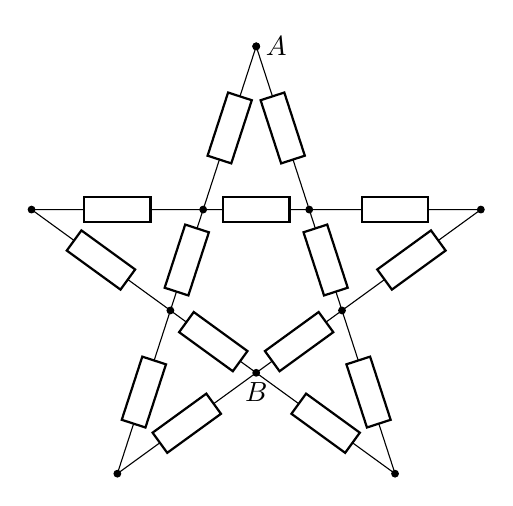
\begin{tikzpicture}[european]

	\coordinate (A1) at (0, 3);
	\coordinate (A2) at (2.8531, 0.92705);
	\coordinate (A3) at (1.7633, -2.4270);
	\coordinate (A4) at (-1.7633, -2.4270);
	\coordinate (A5) at (-2.8531, 0.92705);	

	\coordinate (B1) at (0.67354, 0.92705);
	\coordinate (B2) at (1.08981, -0.354101);
	\coordinate (B3) at (0, -1.1458980);
	\coordinate (B4) at (-1.08981, -0.3541019);
	\coordinate (B5) at (-0.673541, 0.92705);	

	\draw (A1) to [R, *-*, /tikz/circuitikz/bipoles/length=30pt] (B1) to [R,-*, /tikz/circuitikz/bipoles/length=30pt] (A2) to [R,-*, /tikz/circuitikz/bipoles/length=30pt] (B2) to [R,-*, /tikz/circuitikz/bipoles/length=30pt] (A3) to [R,-*, /tikz/circuitikz/bipoles/length=30pt] (B3) to [R,-*, /tikz/circuitikz/bipoles/length=30pt] (A4) to [R,-*, /tikz/circuitikz/bipoles/length=30pt] (B4) to [R,-*, /tikz/circuitikz/bipoles/length=30pt] (A5) to [R,-*, /tikz/circuitikz/bipoles/length=30pt] (B5) to [R,-*, /tikz/circuitikz/bipoles/length=30pt] (A1); 
	\draw (B1) to [R, /tikz/circuitikz/bipoles/length=30pt] (B2) to [R, /tikz/circuitikz/bipoles/length=30pt] (B3) to [R, /tikz/circuitikz/bipoles/length=30pt] (B4) to [R, /tikz/circuitikz/bipoles/length=30pt] (B5) to [R, /tikz/circuitikz/bipoles/length=30pt] (B1);
	\node at (A1) [right] {$A$};
	\node at (B3) [below] {$B$};
\end{tikzpicture}
\end{document}